\documentclass[a4paper,8pt]{article}
\usepackage[utf8]{inputenc}
\usepackage[english]{babel} %language
\usepackage[
backend=bibtex
]{biblatex}
\addbibresource{references.bib}
\usepackage{amssymb}
\usepackage{listings}
\usepackage{xcolor}
\usepackage{array}
\usepackage{float}
\usepackage{amsmath}

%CodeColours
\definecolor{codegreen}{rgb}{0,0.6,0}
\definecolor{codegray}{rgb}{0.5,0.5,0.5}
\definecolor{codepurple}{rgb}{0.58,0,0.82}
\definecolor{backcolour}{rgb}{0.95,0.95,0.92}
\definecolor{codeblue}{rgb}{0,0,0.80}



%Codestyle
\lstdefinestyle{mystyle}{
	backgroundcolor=\color{backcolour},   
	commentstyle=\color{codegreen},
	keywordstyle=\color{orange},
	numberstyle=\tiny\color{codegray},
	stringstyle=\color{codepurple},
	basicstyle=\ttfamily\footnotesize,
	identifierstyle=\color{codeblue},
	breakatwhitespace=false,         
	breaklines=true,                 
	captionpos=b,                    
	keepspaces=true,                 
	numbers=left,                    
	numbersep=5pt,                  
	showspaces=false,                
	showstringspaces=false,
	showtabs=false,                  
	tabsize=2,
	basicstyle=\scriptsize
}
%Set style
\lstset{style=mystyle}

%Images and similar
\usepackage{graphicx}
\graphicspath{.}

%timeline
\usepackage{tikz}
\usetikzlibrary{snakes}
\usepackage{rotating}

\title{Title}
\author{Simon dos Reis Spedsbjerg}

\newcommand{\Phases}{7 }
\newcommand{\phaseq}{Research}
\newcommand{\phasew}{Data Collection}
\newcommand{\phasee}{Analysis}
\newcommand{\phaser}{Design}
\newcommand{\phaset}{Implementation}
\newcommand{\phasey}{Software Verification}
\newcommand{\phaseu}{Scientific Verification}

\usepackage{biblatex}

\begin{document}
	\maketitle
	
	\section{Problem}
	As data collection forever increases and systems ever becomes more depended on the quality of the data. Faulty data may damage the quality of analysis which is performed on the data, and outlier data may indicate another system is failing or an uncommon phenomenon has occurred on the sampled group. Anomalies has become an interest in many sectors, Mukherjee, A\cite{MUKHERJEE2024102444} cite transport, manufactoring, water and power making use of IOT-based sensing.
	
	\section{Project}
	The projects goal is to develop a new system which detect anomalies based on different variables dependencies on each other. As a variable value changes, its change may be a reflection of an error on another variable. As a web of variables all connected, the program should be able to pinpoint the problem area based on the afflicted variables, to the degree of affliction and the spread of the affliction. The projects goal is to develop the product, compare it to similar solutions in the aspect of speed, accuracy, ANDRE TING INDENFOR EMNET SÅSOM TRUE-FALSE RATIO through relevant analysis methods. Determining the pros and cons of this system or any algorithms developed for it compared to state of the art systems or algorithms, may further possible future solutions for software problems.
	
	There is two types of anomalies which the system intends to handle, the normal anomaly which is a one off anomaly which is rare or just a misreading, the other is a discord which is a reaccuring anomaly which can indicate a fault, failure or special event at some point in the observed systems. By the different sensors variables having relations among one another, it is hoped that discords can be determined with high accuracy and precision.
	
	\subsection{Expected Challenges}
		throughout the project I expect that I would have to find solutions for the following challenges.
		\begin{itemize}
			\item Making the system be able to differentiate between a anomaly and a discord with a small sample size.
			\item Determining whether to focus on supervised learning, unsupervised learning or both.
			\item Availbility of data which has the quality required for this project. Either it is successful to gain such data, or a virtual twin of machines which this system would function with has to be made.
		\end{itemize}
	\subsection{Phases}
	We intend to go into \Phases phases during this project.
		\begin{itemize}
			\item \phaseq, develop a clear and thorough understanding of the current state of research in anomaly detection and fault detection and diagnosis by creating a systematic literature review of the subjects.
			\item \phasew, Collect or create relevant data depending on the results of the \phaseq which is relevant to the subject. As the results will be drawn on the solutions ability to handle the data, the quality of the data has a high impact on the project.
			\item \phasee, analyse the problem and with the help of software engineering methods based on the \phaseq \space results.
			\item \phaser, design a theoretical solution to the problem specified in the \phasee with software engineering methods.
			\item \phaset, develop the project based on the results of the \phasee and \phaser using software engineering methods.
			\item \phasey, verify that the solution successfully conforms to the requirements determined in the \phasee and implements all critical features.
			\item \phasey, verify the results from the project and check if it full fills the hypothesis. From this draw a conclusion.
		\end{itemize}
	
	\newpage
	In the following, we see the expected timeline for the project.\newline
	%Timeline
	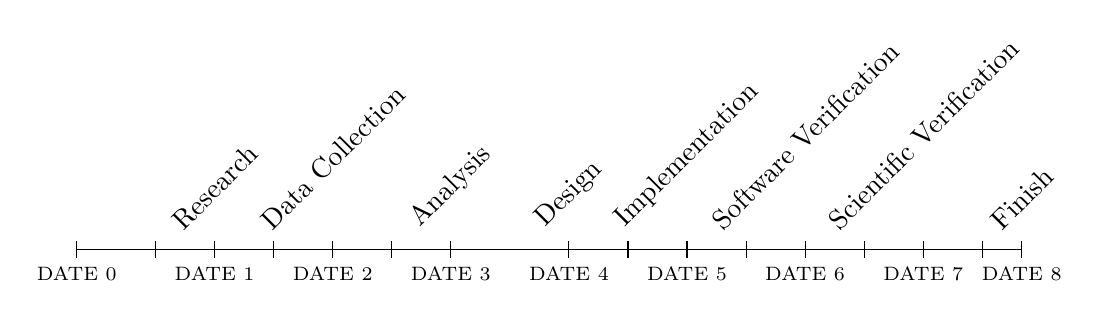
\begin{tikzpicture}
		%create the line
		\draw (-6,0) -- (6,0);
		
		%vertical lines
		\foreach \x in {-6, -5, -4.25, -3.5, -2.75, -2, -1.25, -05, 0.25, 1, 1.75, 2.5, 3.25, 4, 4.75, 5.5, 6}
		\draw (\x cm, 3pt) -- (\x cm, -3pt); %Size of the points in the timeline
		
		%draw
		\draw (-6,0) node[below=3pt] {\scriptsize DATE 0}; node[above=3pt] {$ $}; %start date
		
		\draw (-4.25,0)
		node[below=3pt] {\scriptsize DATE 1}
		node[above=3pt] {\begin{turn}{45}\phaseq\end{turn}};
		
		\draw (-2.75,0)
		node[below=3pt] {\scriptsize DATE 2}
		node[above=3pt] {\begin{turn}{45}
				\phasew
		\end{turn}};
		
		\draw (-1.25,0)
		node[below=3pt] {\scriptsize DATE 3}
		node[above=3pt] {\begin{turn}{45}
				\phasee
		\end{turn}};
		
		\draw (0.25,0)
		node[below=3pt] {\scriptsize DATE 4}
		node[above=3pt] {\begin{turn}{45}
				\phaser
		\end{turn}};
		
		\draw (1.75,0)
		node[below=3pt] {\scriptsize DATE 5}
		node[above=3pt] {\begin{turn}{45}
				\phaset
		\end{turn}};
		
		\draw (3.25,0)
		node[below=3pt] {\scriptsize DATE 6}
		node[above=3pt] {\begin{turn}{45}
				\phasey
		\end{turn}};
		
		\draw (4.75,0)
		node[below=3pt] {\scriptsize DATE 7}
		node[above=3pt] {\begin{turn}{45}
				\phaseu
		\end{turn}};
	
		\draw (6,0) node[below=3pt]{\scriptsize DATE 8} node[above=3pt] {\begin{turn}{45} Finish \end{turn}};%end date
	\end{tikzpicture}
	
	\newpage
	\printbibliography
\end{document}